\documentclass{article}
\usepackage{tikz}
\usetikzlibrary{positioning} % L A T E X and plain T E X
\usetikzlibrary{shapes,backgrounds,fit,decorations,quotes}
\usetikzlibrary{curvilinear}
\begin{document}
\setcounter{section}{16}
\section{Nodes and Edges}
\subsection{nodes and their shapes}

\tikz \fill [fill=yellow!80!black]
(0,0) node {first node}
-- (1,1) node[behind path] {second node}
-- (2,0) node {third node};


\subsection{node contents}
\tikz {
\path (0,0) node [red] {A}
(1,0) node [blue] {B}
(2,0) node [green, node contents=C]
(3,0) node [node contents=D] ;
}

\subsubsection{behind path}
\tikz \fill [fill=blue!50, draw=blue, very thick]
(0,0) node [behind path, fill=red!50] {first node}
-- (1.5,0) node [behind path, fill=green!50] {second node}
-- (1.5,1) node [behind path, fill=brown!50] {third node}
-- (0,1) node [ fill=blue!30] {fourth node};

\tikz \fill[fill=yellow!80!black]
(0,0) node {first node}
-- (1,1) node[ellipse,draw, behind path] {second node}
-- (0,2) node[circle,fill=red!20] {third node};

\subsubsection{Predefined Shapes}
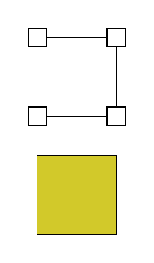
\begin{tikzpicture}[every node/.style={draw}]
\path[yshift=1.5cm,shape=rectangle]
(0,0) node(a1){} (1,0) node(a2){}
(1,1) node(a3){} (0,1) node(a4){};
\filldraw[fill=yellow!80!black] (a1) -- (a2) -- (a3) -- (a4);
\path[shape=coordinate]
(0,0) coordinate(b1) (1,0) coordinate(b2)
(1,1) coordinate(b3) (0,1) coordinate(b4);
\filldraw[fill=yellow!80!black] (b1) -- (b2) -- (b3) -- (b4);
\end{tikzpicture}

\subsubsection{Common Options: Separations, Margins, Padding and Border Rotation}
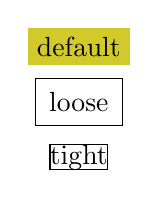
\begin{tikzpicture}
\draw (0,0) node[inner sep=0pt,draw] {tight}
(0cm,2em) node[inner sep=5pt,draw] {loose}
(0cm,4em) node[fill=yellow!80!black] {default};
\end{tikzpicture}

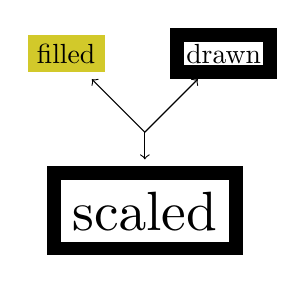
\begin{tikzpicture}
\draw[line width=5pt]
(0,0) node[fill=yellow!80!black] (f) {filled}
(2,0) node[draw] (d) {drawn}
(1,-2) node[draw,scale=2] (s) {scaled};
\draw[->] (1,-1) -- (f);
\draw[->] (1,-1) -- (d);
\draw[->] (1,-1) -- (s);
\end{tikzpicture}

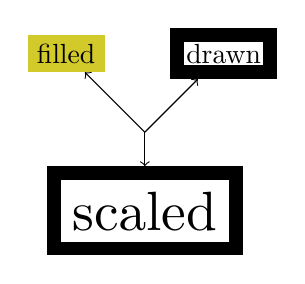
\begin{tikzpicture}[outer sep=auto]
\draw[line width=5pt]
(0,0) node[fill=yellow!80!black] (f) {filled}
(2,0) node[draw] (d) {drawn}
(1,-2) node[draw,scale=2] (s) {scaled};
\draw[->] (1,-1) -- (f);
\draw[->] (1,-1) -- (d);
\draw[->] (1,-1) -- (s);
\end{tikzpicture}

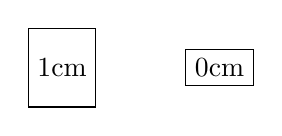
\begin{tikzpicture}
\draw (0,0) node[minimum height=1cm,draw] {1cm}
(2,0) node[minimum height=0cm,draw] {0cm};
\end{tikzpicture}

\begin{tikzpicture}
\draw (0,0) node[minimum height=2cm,minimum width=3cm,draw] {$3 \times 2$};
\end{tikzpicture}
\\
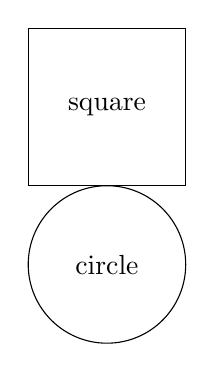
\begin{tikzpicture}
\draw (0,0) node[minimum size=2cm,draw] {square};
\draw (0,-2) node[minimum size=2cm,draw,circle] {circle};
\end{tikzpicture}

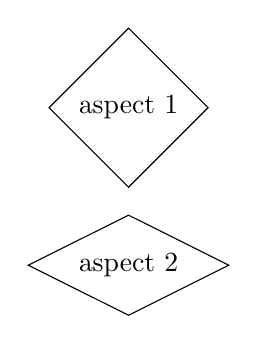
\begin{tikzpicture}
\draw (0,0) node[shape aspect=1,diamond,draw] {aspect 1};
\draw (0,-2) node[shape aspect=2,diamond,draw] {aspect 2};
\end{tikzpicture}


\tikz \tikzset{every node/.style={dart, shape border uses incircle,
inner sep=1pt, draw}}\node foreach \a/\b/\c in {A/0/0, B/45/0, C/0/45, D/45/45}
[shape border rotate=\b, rotate=\c] at (\b/36,-\c/36) {\a};

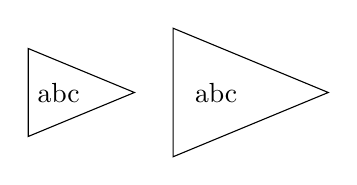
\begin{tikzpicture}
\tikzset{every node/.style={isosceles triangle, draw}}
\node {abc};
\node [shape border uses incircle] at (2,0) {abc};
\end{tikzpicture}

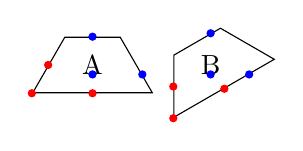
\begin{tikzpicture}
\tikzset{every node/.style={shape=trapezium, draw, shape border uses incircle}}
\node at (0,0) (A) {A};
\node [shape border rotate=30] at (1.5,0) (B) {B};
\foreach \s/\t in
{left side/base east, bottom side/north, bottom left corner/base}{
\fill[red] (A.\s) circle(1.5pt) (B.\s) circle(1.5pt);
\fill[blue] (A.\t) circle(1.5pt) (B.\t) circle(1.5pt);
}
\end{tikzpicture}

\subsection{Multi-Part Nodes}
\subsubsection{node part}
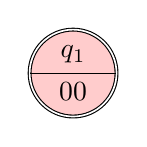
\begin{tikzpicture}
\node [circle split,draw,double,fill=red!20]
{
% No \nodepart has been used, yet. So, the following is put in the
% ``text'' node part by default.
$q_1$
\nodepart{lower} % Ok, end ``text'' part, start ``output'' part
$00$
}; % output part ended.
\end{tikzpicture}


\tikz [every lower node part/.style={red}]
\node [circle split,draw] {$q_1$ \nodepart{lower} $00$};

\subsection{The Node Text}
\subsubsection{Text Parameters: Color and Opacity}
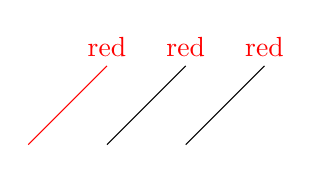
\begin{tikzpicture}
\draw[red] (0,0) -- +(1,1) node[above] {red};
\draw[text=red] (1,0) -- +(1,1) node[above] {red};
\draw (2,0) -- +(1,1) node[above,red] {red};
\end{tikzpicture}

\subsubsection{Text Parameters: Font}
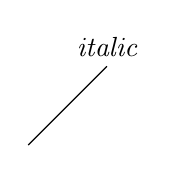
\begin{tikzpicture}
\draw[node font=\itshape] (1,0) -- +(1,1) node[above] {italic};
\end{tikzpicture}

\tikz \node [node font=\tiny, minimum height=3em, draw] {tiny};
\tikz \node [node font=\small, minimum height=3em, draw] {small};


\begin{tikzpicture}
\node [font=\itshape] {italic};
\end{tikzpicture}

\tikz \node [font=\tiny, minimum height=3em, draw] {tiny};
\tikz \node [font=\small, minimum height=3em, draw] {small};

\tikz [every text node part/.style={font=\itshape},
every lower node part/.style={font=\footnotesize}]
\node [circle split,draw] {state \nodepart{lower} output};

\subsubsection{Text Parameters: Alignment and Width for Multi-Line Text}
\tikz \node [draw] {
\begin{tabular}{cc}
upper left & upper right\\
lower left & lower right
\end{tabular}
};

\tikz[align=left] \node[draw] {This is a\\demonstration.};

\tikz \node[fill=yellow!80!black,align=right]
{This is a\\[-2pt] demonstration text for\\[1ex] alignments.};

\tikz \draw (0,0) node[fill=yellow!80!black,text width=3cm]
{This is a demonstration text for showing how line breaking works.};

\tikz \node[fill=yellow!80!black,align=left]
{This is a\\ demonstration text for\\ alignments.};

\tikz (0,0)\node[fill=yellow!80!black,align=left]
{This is a\\ demonstration text for\\ alignments.};

\tikz \node[fill=yellow!80!black,text width=3cm,align=left]
{This is a demonstration text for showing how line breaking works.};

\tikz \node[fill=yellow!80!black,text width=3cm,align=flush left]
{This is a demonstration text for showing how line breaking works.};

\tikz \node[fill=yellow!80!black,align=right]
{This is a\\ demonstration text for\\ alignments.};

\tikz \node[fill=yellow!80!black,align=center]
{This is a\\ demonstration text for\\ alignments.};


\subsection{Positioning Nodes}
\subsubsection{Positioning Nodes Using Anchors}
\tikz \draw (0,0) node[anchor=north east] {first node}
rectangle (1,1) node[anchor=west] {second node};

\subsubsection{Basic Placement Options}
\tikz \fill (0,0) circle (2pt) node[above] {above};

\tikz \fill (0,0) circle (2pt) node[above=2pt] {above};

\tikz \fill (0,0) circle (2pt) node[above left] {above left};

\tikz \fill (0,0) circle (2pt) node[above right] {above right};

\subsubsection{Advanced Placement Options}
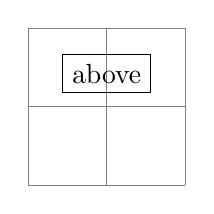
\begin{tikzpicture}
\draw[help lines] (0,0) grid (2,2);
\node at (1,1) [above=2pt+3pt,draw] {above};
\end{tikzpicture}

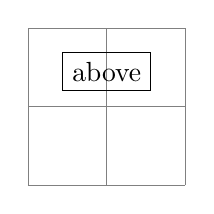
\begin{tikzpicture}
\draw[help lines] (0,0) grid (2,2);
\node at (1,1) [above=.2,draw] {above};
% south border of the node is now 2mm above (1,1)
\end{tikzpicture}

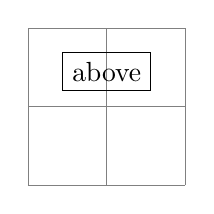
\begin{tikzpicture}
\draw[help lines] (0,0) grid (2,2);
\node at (1,1) [above=.2 and 3mm,draw] {above};
% south border of the node is also 2mm above (1,1)
\end{tikzpicture}

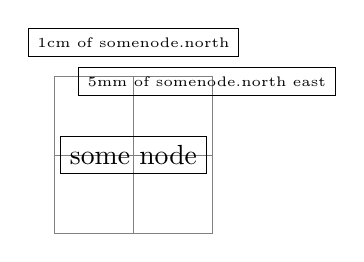
\begin{tikzpicture}[every node/.style=draw]
\draw[help lines] (0,0) grid (2,2);
\node (somenode) at (1,1) {some node};
\node [above=5mm of somenode.north east] {\tiny 5mm of somenode.north east};
\node [above=1cm of somenode.north] {\tiny 1cm of somenode.north};
\end{tikzpicture}

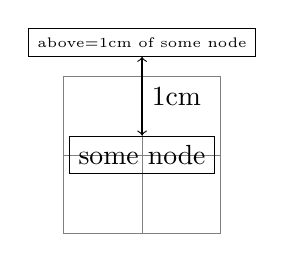
\begin{tikzpicture}[every node/.style=draw]
\draw[help lines] (0,0) grid (2,2);
\node (some node) at (1,1) {some node};
\node (other node) [above=1cm of some node] {\tiny above=1cm of some node};
\draw [<->] (some node.north) -- (other node.south)
node [midway,right,draw=none] {1cm};
\end{tikzpicture}

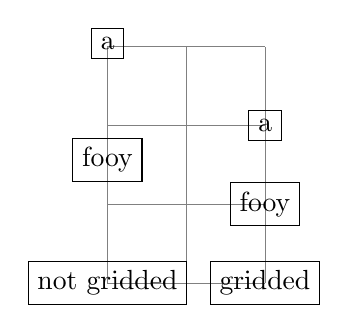
\begin{tikzpicture}[every node/.style=draw]
\draw[help lines] (0,0) grid (2,3);
% Not gridded
\node (a1) at (0,0) {not gridded};
\node (b1) [above=1cm of a1] {fooy};
\node (c1) [above=1cm of b1] {a};
% gridded
\node (a2) at (2,0) {gridded};
\node (b2) [on grid,above=1cm of a2] {fooy};
\node (c2) [on grid,above=1cm of b2] {a};
\end{tikzpicture}

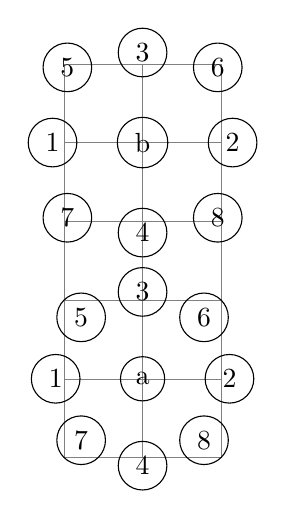
\begin{tikzpicture}[every node/.style={draw,circle}]
\draw[help lines] (0,0) grid (2,5);
\begin{scope}[node distance=5mm and 5mm]
\node (b) at (1,4) {b};
\node [left=of b] {1}; \node [right=of b] {2};
\node [above=of b] {3}; \node [below=of b] {4};
\node [above left=of b] {5}; \node [above right=of b] {6};
\node [below left=of b] {7}; \node [below right=of b] {8};
\end{scope}
\begin{scope}[node distance=5mm]
\node (a) at (1,1) {a};
\node [left=of a] {1}; \node [right=of a] {2};
\node [above=of a] {3}; \node [below=of a] {4};
\node [above left=of a] {5}; \node [above right=of a] {6};
\node [below left=of a] {7}; \node [below right=of a] {8};
\end{scope}
\end{tikzpicture}


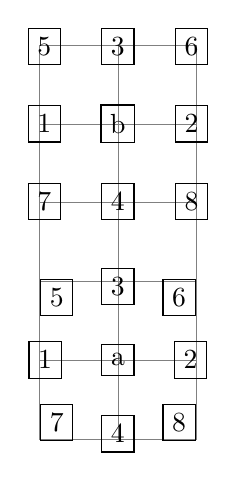
\begin{tikzpicture}[every node/.style={draw,rectangle}]
\draw[help lines] (0,0) grid (2,5);
\begin{scope}[node distance=5mm and 5mm]
\node (b) at (1,4) {b};
\node [left=of b] {1}; \node [right=of b] {2};
\node [above=of b] {3}; \node [below=of b] {4};
\node [above left=of b] {5}; \node [above right=of b] {6};
\node [below left=of b] {7}; \node [below right=of b] {8};
\end{scope}
\begin{scope}[node distance=5mm]
\node (a) at (1,1) {a};
\node [left=of a] {1}; \node [right=of a] {2};
\node [above=of a] {3}; \node [below=of a] {4};
\node [above left=of a] {5}; \node [above right=of a] {6};
\node [below left=of a] {7}; \node [below right=of a] {8};
\end{scope}
\end{tikzpicture}

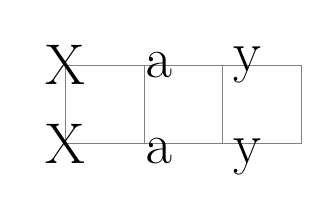
\begin{tikzpicture}[node distance=1ex]
\draw[help lines] (0,0) grid (3,1);
\huge
\node (X) at (0,1) {X};
\node (a) [right=of X] {a};
\node (y) [right=of a] {y};
\node (X) at (0,0) {X};
\node (a) [base right=of X] {a};
\node (y) [base right=of a] {y};
\end{tikzpicture}

\subsection{Fitting Nodes to a Set of Coordinates}
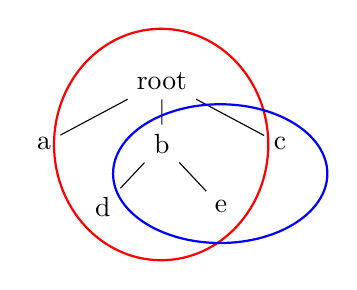
\begin{tikzpicture}[level distance=8mm]
\node (root) {root}
child { node (a) {a} }
child { node (b) {b}
child { node (d) {d} }
child { node (e) {e} } }
child { node (c) {c} };
\node[draw=red,inner sep=0pt,thick,ellipse,fit=(root) (b) (d) (e)] {};
\node[draw=blue,inner sep=0pt,thick,ellipse,fit=(b) (c) (e)] {};
\end{tikzpicture}

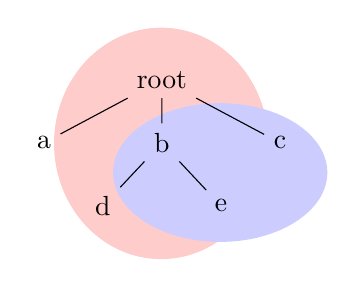
\begin{tikzpicture}[level distance=8mm]
\node (root) {root}
child { node (a) {a} }
child { node (b) {b}
child { node (d) {d} }
child { node (e) {e} } }
child { node (c) {c} };
\begin{scope}[on background layer]
\node[fill=red!20,inner sep=0pt,ellipse,fit=(root) (b) (d) (e)] {};
\node[fill=blue!20,inner sep=0pt,ellipse,fit=(b) (c) (e)] {};
\end{scope}
\end{tikzpicture}

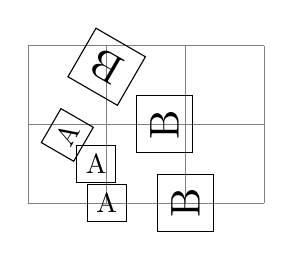
\begin{tikzpicture}[every node/.style={draw}]
\draw[help lines](0,0) grid (3,2);
\draw (1,0) node{A}
(2,0) node[rotate=90,scale=1.5] {B};
\draw[rotate=30] (1,0) node{A}
(2,0) node[rotate=90,scale=1.5] {B};
\draw[rotate=60] (1,0) node[transform shape] {A}
(2,0) node[transform shape,rotate=90,scale=1.5] {B};
\end{tikzpicture}

\tikz \draw (0,0) -- (3,1)
node[pos=0]{0} node[pos=0.5]{1/2} node[pos=0.9]{9/10};

\tikz \draw (0,0) .. controls +(right:3.5cm) and +(right:3.5cm) .. (0,3)
node foreach \p in {0,0.125,...,1} [pos=\p]{\p};

\tikz \draw (0,0) |- (3,1)
node[pos=0]{0} node[pos=0.5]{1/2} node[pos=0.9]{9/10};

\tikz \draw (0,0) -| (3,1)
node[pos=0]{0} node[pos=0.5]{1/2} node[pos=0.9]{9/10};

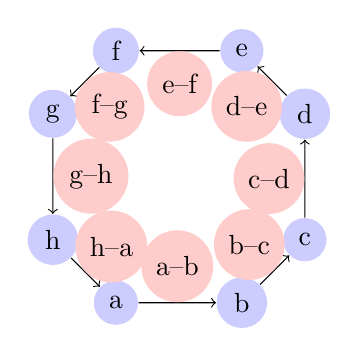
\begin{tikzpicture}
[scale=.8,auto=left,every node/.style={circle,fill=blue!20}]
\node (a) at (-1,-2) {a};
\node (b) at ( 1,-2) {b};
\node (c) at ( 2,-1) {c};
\node (d) at ( 2, 1) {d};
\node (e) at ( 1, 2) {e};
\node (f) at (-1, 2) {f};
\node (g) at (-2, 1) {g};
\node (h) at (-2,-1) {h};
\foreach \from/\to in {a/b,b/c,c/d,d/e,e/f,f/g,g/h,h/a}
\draw [->] (\from) -- (\to)
node[midway,fill=red!20] {\from--\to};
\end{tikzpicture}


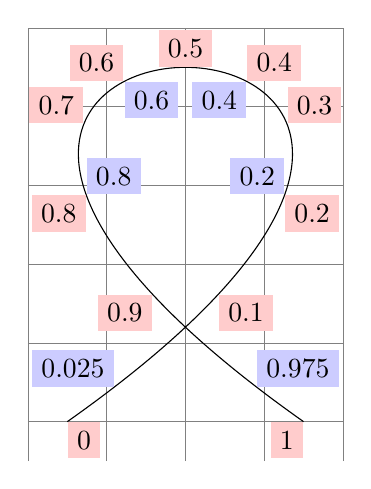
\begin{tikzpicture}[auto]
\draw[help lines,use as bounding box] (0,-.5) grid (4,5);
\draw (0.5,0) .. controls (9,6) and (-5,6) .. (3.5,0)
node foreach \pos in {0,0.1,0.2,0.3,0.4,0.5,0.6,0.7,0.8,0.9,1}
[pos=\pos,swap,fill=red!20] {\pos}
node foreach \pos in {0.025,0.2,0.4,0.6,0.8,0.975}
[pos=\pos,fill=blue!20] {\pos};
\end{tikzpicture}

\tikz \draw (0,0) .. controls +(up:2cm) and +(left:2cm) .. (1,3)
node foreach \p in {0,0.25,...,1} [sloped,above,pos=\p]{\p};


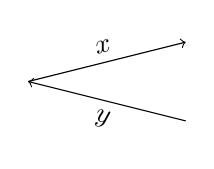
\begin{tikzpicture}[->]
\draw (0,0) -- (2,0.5) node[midway,sloped,above] {$x$};
\draw (2,-.5) -- (0,0) node[midway,sloped,below] {$y$};
\end{tikzpicture}

\tikz [allow upside down]
\draw (0,0) .. controls +(up:2cm) and +(left:2cm) .. (1,3)
node foreach \p in {0,0.25,...,1} [sloped,above,pos=\p]{\p};

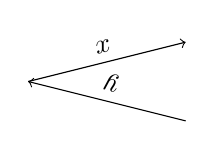
\begin{tikzpicture}[->,allow upside down]
\draw (0,0) -- (2,0.5) node[midway,sloped,above] {$x$};
\draw (2,-.5) -- (0,0) node[midway,sloped,below] {$y$};
\end{tikzpicture}

\tikz \draw (0,0) .. controls +(up:2cm) and +(left:3cm) .. (1,5)
node[at end] {\texttt{at end}}
node[very near end] {\texttt{very near end}}
node[near end] {\texttt{near end}}
node[midway] {\texttt{midway}}
node[near start] {\texttt{near start}}
node[very near start] {\texttt{very near start}}
node[at start] {\texttt{at start}};

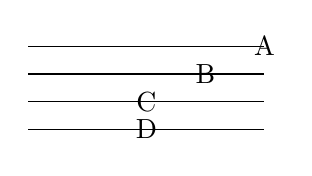
\begin{tikzpicture}[near end]
\draw (0cm,4em) -- (3cm,4em) node{A};
\draw (0cm,3em) -- node{B} (3cm,3em);
\draw (0cm,2em) -- node[midway] {C} (3cm,2em);
\draw (0cm,1em) -- (3cm,1em) node[midway] {D} ;
\end{tikzpicture}

\subsection{The Label and Pin Options}
\tikz [circle] {
\node [draw] (s) {};
\node [draw] (a) [right=of s] {} edge (s);
\node [draw] (b) [right=of a] {} edge (a);
\node [draw] (t) [right=of b] {} edge (b);
}

\tikz [circle] {
\node [draw] (s) [label=$s$] {};
\node [draw] (a) [right=of s] {} edge (s);
\node [draw] (b) [right=of a] {} edge (a);
\node [draw] (t) [right=of b, label=$t$] {} edge (b);
}

\tikz [rotate=-80,every label/.style={draw,red}]
\node [transform shape,rectangle,draw,label=right:label] {main node};

\tikz [rotate=-80,every label/.style={draw,red},absolute]
\node [transform shape,rectangle,draw,label=right:label] {main node};

\tikz
\node [circle, draw,
label=default,
label=60:$60^\circ$,
label=below:$-90^\circ$,
label=3:$3^\circ$,
label=2:$2^\circ$,
label={[below]180:$180^\circ$},
label={[centered]135:$135^\circ$}] {my circle};

\tikz \node [transform shape,rotate=90,
rectangle,draw,label={[red]center:R}] {main node};

\tikz \node [circle,draw,label={[red]above:X}] {my circle};

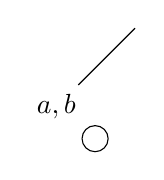
\begin{tikzpicture}
\node [circle,draw,label={[name=label node]above left:$a,b$}] {};
\draw (label node) -- +(1,1);
\end{tikzpicture}

\tikz[label distance=5mm]
\node [circle,draw,label=right:X,
label=above right:Y,
label=above:Z] {my circle};



\tikz \node [circle,fill=blue!50,minimum size=1cm,pin=60:$q_0$] {};

\tikz[pin distance=1cm]
\node [circle,draw,pin=right:X,
pin=above right:Y,
pin=above:Z] {my circle};

\tikz[pin distance=10mm]
\node [circle,draw,pin={[pin edge={blue,thick}]right:X},
pin=above:Z] {my circle};

\tikz[pin distance=10mm]
\node [circle,draw,pin={[pin edge={blue,thick}]right:X},
pin=above:Z] {my circle};

\tikz [every pin edge/.style={},
initial/.style={pin={[pin distance=5mm,
pin edge={<-,shorten <=1pt}]left:start}}]
\node [circle,draw,initial] {my circle};

\tikz \node ["my label" red, draw] {my node};

\tikz \node [label={[red]my label}, draw] {my node};

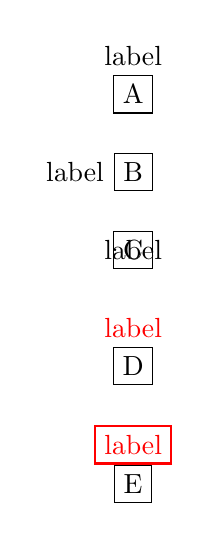
\begin{tikzpicture}
\matrix [row sep=5mm] {
\node [draw, "label"] {A}; \\
\node [draw, "label" left] {B}; \\
\node [draw, "label" centered] {C}; \\
\node [draw, "label" color=red] {D}; \\
\node [draw, "label" {red,draw,thick}] {E}; \\
};
\end{tikzpicture}

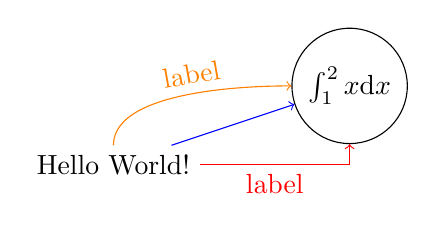
\begin{tikzpicture}
\path (0,0) node (x) {Hello World!}
(3,1) node[circle,draw](y) {$\int_1^2 x \mathrm d x$};
\draw[->,blue] (x) -- (y);
\draw[->,red] (x) -| node[near start,below] {label} (y);
\draw[->,orange] (x) .. controls +(up:1cm) and +(left:1cm) .. node[above,sloped] {label} (y);
\end{tikzpicture}

\subsection{Connecting Nodes: Using the Edge Operation}
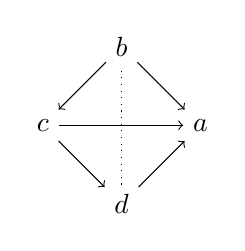
\begin{tikzpicture}
\node (a) at (0:1) {$a$};
\node (b) at (90:1) {$b$} edge [->] (a);
\node (c) at (180:1) {$c$} edge [->] (a)
edge [<-] (b);
\node (d) at (270:1) {$d$} edge [->] (a)
edge [dotted] (b)
edge [<-] (c);
\end{tikzpicture}

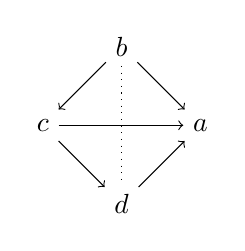
\begin{tikzpicture}
\node foreach \name/\angle in {a/0,b/90,c/180,d/270}
(\name) at (\angle:1) {$\name$};
\path[->] (b) edge (a)
edge (c)
edge [-,dotted] (d)
(c) edge (a)
edge (d)
(d) edge (a);
\end{tikzpicture}

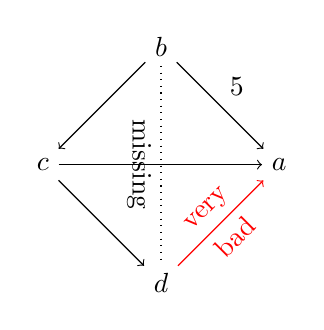
\begin{tikzpicture}
\node foreach \name/\angle in {a/0,b/90,c/180,d/270}
(\name) at (\angle:1.5) {$\name$};
\path[->] (b) edge node[above right] {$5$} (a)
edge (c)
edge [-,dotted] node[below,sloped] {missing} (d)
(c) edge (a)
edge (d)
(d) edge [red] node[above,sloped] {very}
node[below,sloped] {bad} (a);
\end{tikzpicture}

\begin{tikzpicture}[every edge/.style={draw,dashed}]
\path (0,0) edge (3,2);
\end{tikzpicture}

\tikz \draw (0,0) edge ["left", ->] (2,0);

\tikz [every edge quotes/.style={auto=right}]
\draw (0,0) edge ["right", ->] (2,0);

\tikz [every edge quotes/.style={fill=white,font=\footnotesize}]
\draw (0,0) edge ["mid", ->] (2,1);

\tikz
\draw (0,0) edge ["left", "right"',
"start" near start,
"end"' near end] (4,0);

\tikz [tight/.style={inner sep=1pt}, loose/.style={inner sep=.7em}]
\draw (0,0) edge ["left" tight,
"right"' loose,
"start" near start] (4,0);
\end{document}